\documentclass[12pt,fleqn,unicode]{article}
\usepackage{cmap}
\usepackage[utf8]{inputenc}
\usepackage[T1]{fontenc}
\usepackage[russian]{babel}
\usepackage[pdftex]{graphicx}
\usepackage{hyperref}
\usepackage{xcolor}
\usepackage{caption}
\usepackage{pdfpages}
\usepackage{amsmath}
\usepackage{grffile}
\usepackage{amssymb}
\usepackage{hhline}
\usepackage{multicol}
\usepackage[left=2cm, top=2cm, right=2cm, bottom=2cm]{geometry}

\title{Отчет по заданию <<Метод~опорных~векторов>>}
\author{Скачков~Н.А.~317~группа}
\begin{document}
	\maketitle

\section{Введение}
В данном отчете приведено сравнение различных стратегий поиска разделяющей поверхности
методом опорных векторов. Для построения линейных поверхностей решались:
\begin{itemize}
	\item прямая задача SVM~---~методом внутренней точки;
	\item двойственная задача SVM без ядрового перехода~---~методом внутренней точки;
	\item прямая задача SVM~---~методом полного и стохастического градиентных спусков,
		 а также методом PEGASOS.
\end{itemize}

Для построения нелинейных разделяющих поверхностей решались:
\begin{itemize}
	\item двойственная задача SVM с полиномиальным ядром~---~методом внутренней точки;
	\item двойственная задача SVM с RBF ядром~---~методом внутренней точки;
\end{itemize}

Во второй части отчета будет проведено сравнение предложенных методов с использованием
параметров по умолчанию. Для сравнения будут использоваться различные по сложности и
структуре сгенерированные выборки.

В третьей части отчета будет проведен анализ влияния настройки параметров на качество
классификации и форму разделяющей поверхности.

\section{Сравнение различных стратегий}
Проведем сравнение времени работы алгоритмов в зависимости от количества объектов в выборке
(Таблица \ref{tab1}). Сравнение проводилось на линейно неразделимой выборке с 500 признаками,
чтобы алгоритмы не сходились слишком быстро.

Как видно, из методов внутренней точки самыми долгими являются решения прямой задачи и двойственной
с полиномиальным ядром. Для прямой задачи это может быть связано с тем, что число оптимизируемых 
параметров значительно больше чем в двойственных методах. Для двойственной с полиномиальным ядром
это может быть связано с длительностью операции поэлементного возведения в степень матрицы размера
число объектов на число объектов.

\pagebreak
\begin{table}[h!]
	\centering
	\begin{tabular}{|l|c|c|c|c|}
\hline
Алгоритм & 500 & 1000 & 1500 & 2000 \\ \hline
Метод внутренней точки (прямая задача) & 0.8 & 2.1 & 4.5 & 10.3 \\ \hline
Метод внутренней точки (двойственная, без ядра) & 0.2 & 1.2 & 2.9 & 6.7 \\ \hline
Метод внутренней точки (двойственная, RBF ядро) & 0.3 & 1.4 & 2.2 & 5.2 \\ \hline
Метод внутренней точки (двойственная, полином. ядро) & 0.4 & 1.8 & 4.4 & 9.8 \\ \hline
Полный субградиентный спуск & 7.4 & 25.7 & 39.4 & 62.0 \\ \hline
Стохастический субградиентный спуск & 7.1 & 13.5 & 18.0 & 22.4 \\ \hline
Метод PEGASOS & 5.2 & 12.9 & 19.1 & 20.9 \\ \hline
	\end{tabular}
	\caption{Время работы различных стратегий в зависимости от количества объектов,~(c)}
	\label{tab1}
\end{table}

Для субградиентных методов было взято одинаковое количество итераций. 
Видно, что полный градиентный спуск работает значительно дольше других методов, 
что объясняется тем, что время выполнения поиска субградиента на каждой итерации производится по 
всей выборке.

Сравнение времени работы алгоритмов для различного числа признаков приведено в Таблице \ref{tab2}.
Как видно, из методов внутренней точки дольше всех работает решение прямой задачи. Это связано с тем,
что только в ней количество параметров в ней пропорционально количеству признаков.

Для всех субградиентных методов виден схожий рост времени работы алгоритмов, что объясняется тем, что
время подсчета градиента ля всех этих методов растет одинаково, пропорционально числу признаков.

\begin{table}[h!]
	\centering
	\begin{tabular}{|l|c|c|c|c|}
\hline
Алгоритм & 100 & 500 & 1000 & 1500 \\ \hline
Метод внутренней точки (прямая задача) & 2.0 & 3.1 & 5.1 & 9.0 \\ \hline
Метод внутренней точки (двойственная, без ядра) & 1.5 & 1.6 & 1.6 & 1.5 \\ \hline
Метод внутренней точки (двойственная, RBF ядро) & 0.8 & 0.9 & 1.5 & 1.6 \\ \hline
Метод внутренней точки (двойственная, полином. ядро) & 1.9 & 2.0 & 2.0 & 2.0 \\ \hline
Полный субградиентный спуск & 2.0 & 11.6 & 24.3 & 44.6 \\ \hline
Стохастический субградиентный спуск & 3.0 & 13.9 & 23.3 & 37.3 \\ \hline
Метод PEGASOS & 2.2 & 12.5 & 26.8 & 37.7 \\ \hline
	\end{tabular}
	\caption{Время работы различных стратегий в зависимости от количества признаков,~(c)}
	\label{tab2}
\end{table}

Значения целевой функции, к которым сошлись различные методы, можно увидеть в Таблице \ref{tab3}.

\begin{table}[h!]
	\centering
	\begin{tabular}{|l|c|}
\hline
Алгоритм & Значение функции потерь \\ \hline
Метод внутренней точки (прямая задача) & 0.62 \\ \hline
Метод внутренней точки (двойственная, без ядра) & -0.62 \\ \hline
Метод внутренней точки (двойственная, RBF ядро) & -0.98 \\ \hline
Метод внутренней точки (двойственная, полином. ядро) & -0.33 \\ \hline
Полный субградиентный спуск & 0.062 \\ \hline
Стохастический субградиентный спуск & 0.62 \\ \hline
Метод PEGASOS & 0.62 \\ \hline
	\end{tabular}
	\caption{Значение целевой функции для различных методов}
	\label{tab3}
\end{table}

Двойственные задачи имеют, как и ожидалось, отрицательные значения, так как изначально
решается задача максимизации.
Можно заметить, что для всех линейных методов получились одинаковые итоговые значения, а для 
нелинейных~---~другие, так как в них оптимизировался другой функционал.

Характер сходимости можно увидеть на Рисунке \ref{fig1}. Как видно, значение функционала во всех методах
колеблется, и сходимость присутствует только за счет наличия затухания шага во всех субградиентных методах.
Также у полного градиента можно увидеть точку, в которой значение функционала практически перестает меняться
(30 итерация), однако после этого функционал продолжает уменьшаться, увеличив колебания. Это означает, что
есть риск ранней остановки, и лучше делать больше итераций в алгоритмах субградиентного спуска, так как возможно
резкое улучшение после нахождения на <<плато>>~---~области с близким к $0$ значением субградиента.

\begin{figure}[h!]
	\centering
	\caption{Сходимость функций потерь субградиентных методов}
	\label{fig1}
	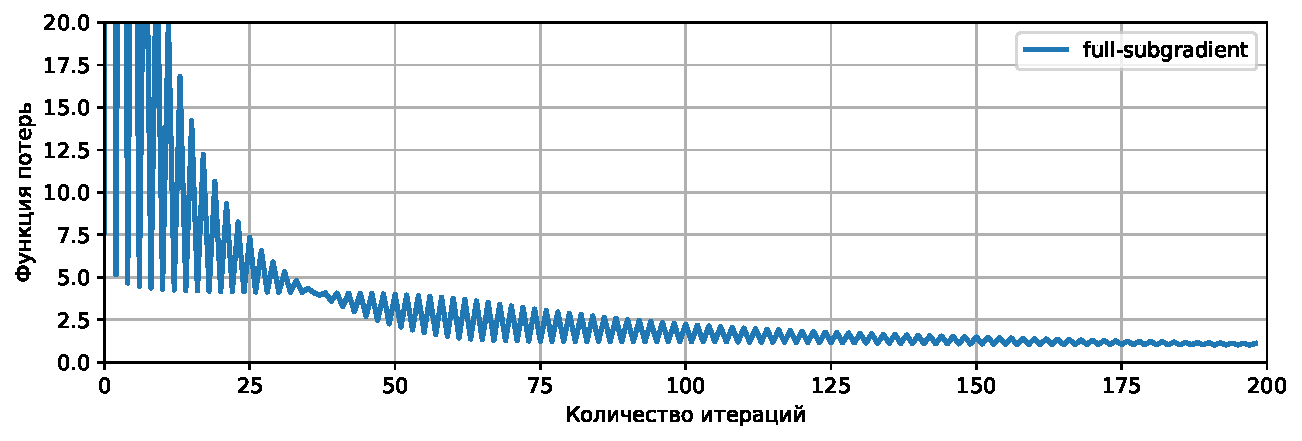
\includegraphics[width=15cm]{../pict/fs.pdf}
	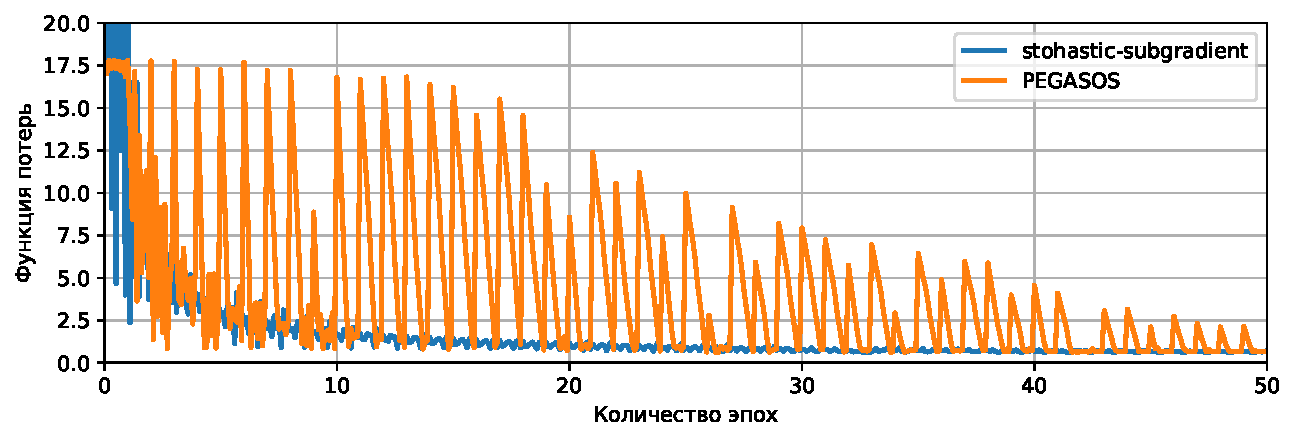
\includegraphics[width=15cm]{../pict/ss.pdf}
\end{figure}

Рассмотрим значения точности различных моделей на искусственных датасетах, обладающих различными свойствами.
(Таблица \ref{tab4}). Были взяты следующие датасеты:
\begin{itemize}
	\item lin-split~---~линейно разделимая выборка;
	\item moons~---~линейно неразделимая выборка, состоящая из непересекающихся классов, сгенерированных
	в форме лун;
	\item non-split~---~выборка, состоящая из частично пересекающихся классов;
	\item outliers~---~линейно разделимая выборка с добавлением 30\% выбросов;
	\item imbalanced~---~ выборка с соотношением классов 2 к 8.
\end{itemize}
\pagebreak

\begin{table}[h!]
	\centering
	\begin{tabular}{|l|c|c|c|c|c|}
\hline
Алгоритм & lin-split & moons & non-split & outliers & imbalanced\\ \hline
SVM, прямая задача & 1.000 & 0.796 & 0.910 & 0.857 & 1.000 \\ \hline
SVM, двойственная, без ядра & 1.000 & 0.783 & 0.842 & 0.857 & 1.000 \\ \hline
SVM, двойственная, RBF ядро & 1.000 & 0.988 & 0.994 & 0.983 & 1.000 \\ \hline
SVM, двойственная, полином. ядро & 1.000 & 0.873 & 0.924 & 0.857 & 1.000 \\ \hline
Полный субградиентный спуск & 1.000 & 0.798 & 0.916 & 0.857 & 0.931 \\ \hline
Стох. субградиентный спуск & 1.000 & 0.796 & 0.908 & 0.857 & 0.970 \\ \hline
Метод PEGASOS & 1.000 & 0.799 & 0.924 & 0.857 & 1.000 \\ \hline
	\end{tabular}
	\caption{Точность разных моделей на различных датасетах}
	\label{tab4}
\end{table}

Можно увидеть, что нелинейные алгоритмы имеют намного более высокие значения точности, что объясняется их
большей сложностью. При этом не исключено переобучение таких моделей. 

Для линейных моделей можно заметить, что
полный субградиентный метод намного сильнее остальных ошибается на несбалансированных классах, что меньше
проявляется для стохастического метода. Также видно, что PEGASOS дает наилучшие из всех линейных методов результаты.

На примере стохастического субградиентного метода, проанализируем связь между точностью на обучающей выборке
и значением функции потерь (Рис. \ref{fig2}).

\begin{figure}[h!]
	\centering
	\caption{Связь функции потерь и точности}
	\label{fig2}
	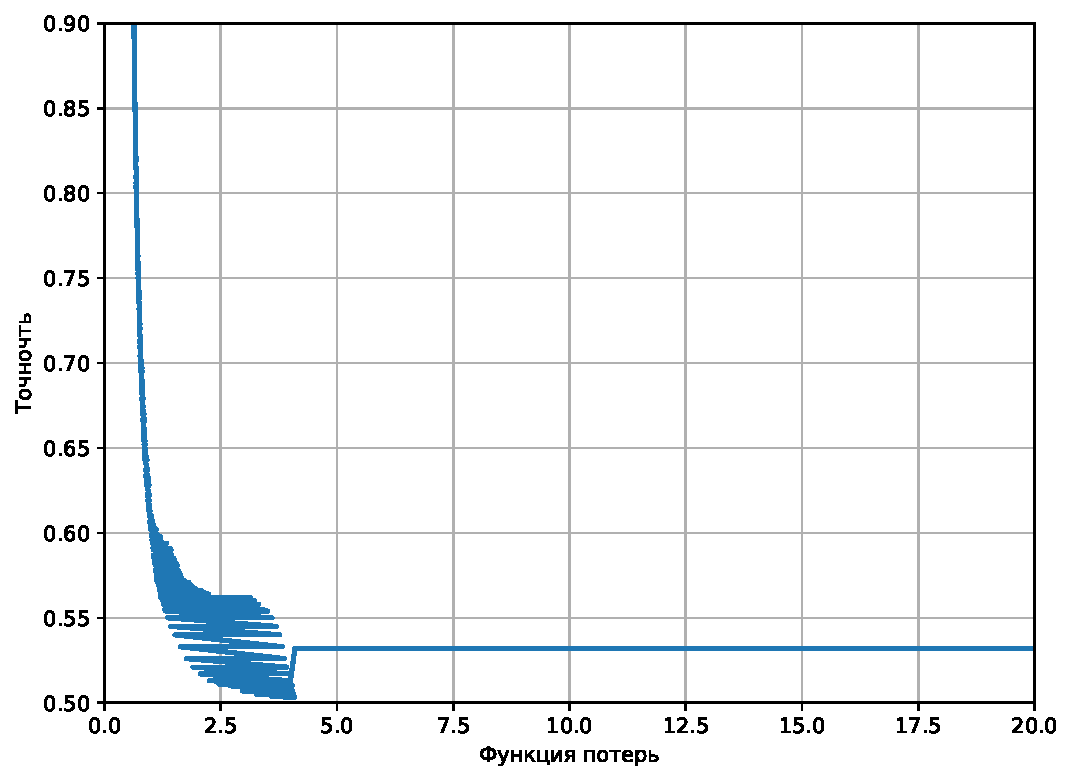
\includegraphics[width=10cm]{../pict/acc-func.pdf}
\end{figure}

Как можно увидеть, низкие значения функционала связаны с высокой точностью, также как высокие значения~---~с низкой
точностью. В остальных случаях зависимости не наблюдается. Можно сделать вывод, что для определения сходимости
достаточно рассматривать лишь один из этих функционалов.

\pagebreak
\section{Настройка параметров}

\subsection{Настройка параметров SVM}

Настроим параметр $C$, общий для всех моделей, решая линейную двойственную задачу. Оценивать модели будем по
кроссвалидации с 5 фолдами по выборке c пересекающимися классами. Значения по всем фолдам будем усреднять.

\begin{table}[h!]
	\centering
	\begin{tabular}{|c|c|c|c|c|c|c|}
	\hline
$C$ & 1 & 5 & 10 & 25 & \textbf{50} & 100 \\ \hline
Точность & 0.763 & 0.836 & 0.851 & 0.864 & \textbf{0.868} & 0.856 \\ \hline
	\end{tabular}
	\caption{Значение точности на кроссвалидации для разных $C$}
	\label{tab5}
\end{table}

Как видно, оптимальное значение достигается при $C=50$, после чего точность начинает падать.

Попробуем подобрать $C$ обучаясь на линейно разделимой выборке (Таблица \ref{tab6}). Тут также
использовалась кроссвалидация с 5 фолдами.

\begin{table}[h!]
	\captionsetup{justification=centering}
	\centering
	\begin{tabular}{|c|c|c|c|c|c|c|}
	\hline
$C$ & 1 & 5 & 10 & 25 & 50 & 100 \\ \hline
Точность & 1.000 & 1.000 & 1.000 & 1.000 & 1.000 & 0.998 \\ \hline
	\end{tabular}
	\caption{Значение точности на кроссвалидации для разных $C$ для линейно~разделимой~выборки}
	\label{tab6}
\end{table}

Как можно заметить, подбор параметра не дал никаких результатов, так как для любых $C$ классификация
идеальна или близка к идеальной.

Подберем параметр $\gamma$ для RBF ядра. На этот раз кроссвалидацию будем проводить только на
выборке с пересекающимися классами (Таблица \ref{tab7}).

\begin{table}[h!]
	\captionsetup{justification=centering}
	\centering
	\begin{tabular}{|c|c|c|c|c|c|c|}
	\hline
$\gamma$ & 1 & \textbf{5} & 10 & 15 \\ \hline
Точность & 0.876 & \textbf{0.877} & 0.873 & 0.870 \\ \hline
	\end{tabular}
	\caption{Значение точности на кроссвалидации для разных $\gamma$}
	\label{tab7}
\end{table}

Как видно, оптимальное значение параметра ширины $\gamma$ равняется 5.

Подберем теперь степень полинома d для полиномиального ядра, использую кроссвалидацию
на том же датасете (Таблица \ref{tab8}).

\begin{table}[h!]
	\captionsetup{justification=centering}
	\centering
	\begin{tabular}{|c|c|c|c|c|c|c|}
	\hline
Степень & 1 & 2 & \textbf{3} & 4 & 5 \\ \hline 
Точность & 0.925 & 0.921 & \textbf{0.937} & 0.935 & 0.935 \\ \hline
	\end{tabular}
	\caption{Значение точности на кроссвалидации для разных $d$}
	\label{tab8}
\end{table}

Заметим, что RBF ядро дает несколько более плохие значения после настройки параметров, 
что связано с тем, что оно строит более сложную поверхность. В итоге эта модель становится
более чувствительной к выбросам и ее обобщающая способность падает.

Также заметим, что хоть выборка и состоит из пересекающихся классов, линейная модель дает достаточно
неплохие результаты, хоть и строит очень простую разделяющую поверхность.

\subsection{Настройка параметров субградиентных методов}

Различные параметры субградиентных методов не меняют функционал качества, но 
влияют на скорость сходимости этих методов, то к чему они сходятся, и сходятся ли они вообще.

Рассмотрим влияние параметра угасания шага субградиентного спуска $\beta$ (Рис. \ref{fig3}).
Здесь и далее оценка параметра производится на выборке с пересекающимися классами, с кроссвалидацией по 
5 фолдам. Значения истории функционала точности для всех батчей усредняются.

\begin{figure}[h!]
	\centering
	\caption{Сходимость стох. субградиентного метода для разных значений параметра $\beta$}
	\label{fig3}
	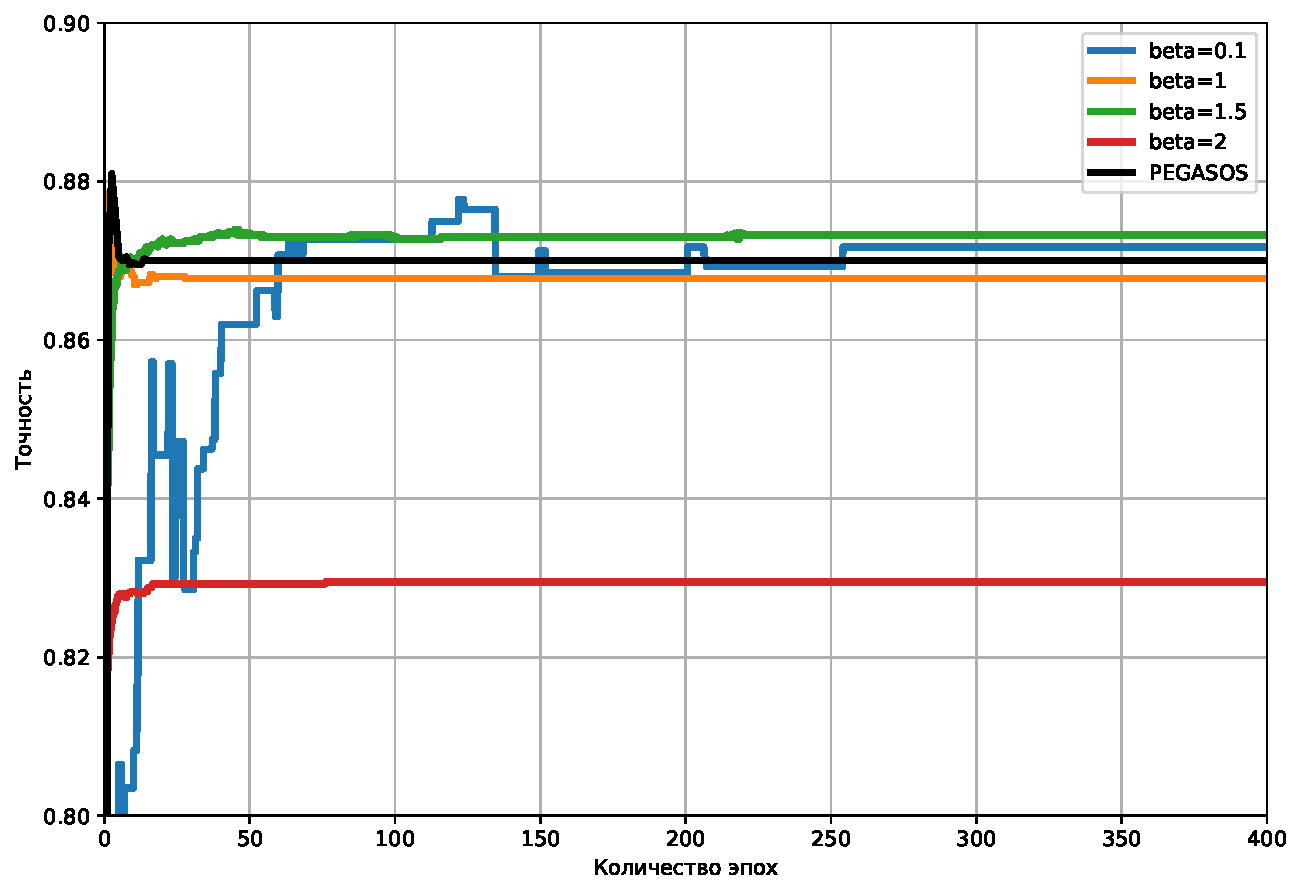
\includegraphics[width=14cm]{../pict/beta.pdf}
\end{figure}

Как видно, наилучшим оказалось значение $\beta = 0.1$, однако метод PEGASOS имеет более высокую точность
и достигает ее намного быстрее.

Значение $\beta = 0$, так же было рассмотрено, однако максимальная точность
на нем была порядка $0.4$ и не была отображена на графике.  Это можно объяснить тем, что в теории 
субградиентный метод не обязан сходиться, и чтобы метод обладал этим свойством необходимо, чтобы величина шага
уменьшалась с итерациями.

В целом можно сказать, что сходимость субградиентного метода неустойчива и при попадании в оптимальное значение
алгоритм может легко из него уйти.

Рассмотрим теперь характер сходимости для различных размеров батчей (Рис. \ref{fig4}). <<Базовое>> значение 
точности, полученное с помощью решения двойственной задачи методом внутренней точки, показано на графике
пунктиром.

Можно увидеть, что увеличение числа объектов в батче ухудшает качество классификации. Это может объясняться тем,
что алгоритм достаточно нестабилен, и при малых значениях батча больше вероятность того, что метод случайно попадет
ближе к оптимуму.

Заметим также, что при наилучшем параметре размера батча, равном $100$, алгоритм дал лучший результат, чем
решение методом внутренней точки.

\pagebreak

\begin{figure}[h!]
	\centering
	\caption{Сходимость стохастического субградиентного метода для различных размеров батчей}
	\label{fig4}
	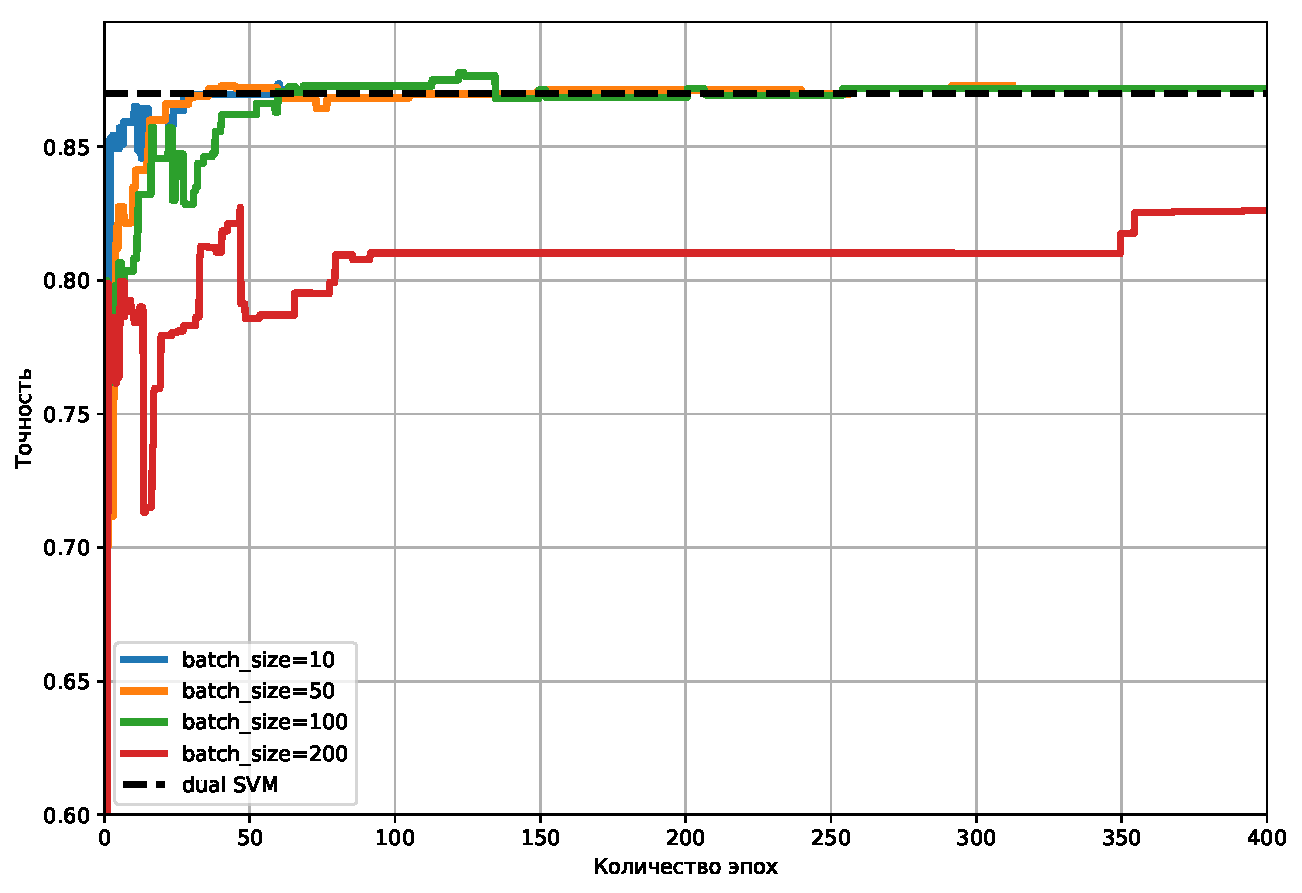
\includegraphics[width=14cm]{../pict/bs.pdf}
\end{figure}

Сравним результаты подбора параметров с результатами, полученными для градиентных методов в задаче
логистической регрессии.

В градиентных методах увеличение размера батча зачастую приводило к улучшению качества модели, увеличивая
лишь время работы метода. В субградиентных методах большая величина батча ухудшает итоговое качество, так 
как уменьшается вероятность попадания в оптимум.

Параметр угасания шага $\beta$ в градиентных методах влиял только на скорость сходимости методов и лишь
немного улучшал качество. В субградиентных методах этот параметр является обязательным, так как без него 
метод вообще не сходится.

Характер сходимости у градиентных и субградиентных методов также различается. Градиентные методы сходятся 
монотонно, без скачков. В субградиентных, наоборот, требуется смотреть лучшее значение, полученное за время
работы метода. Сходимость немонотонная, присутствуют резкие скачки функционалов качества.

Субградиентный метод стоит использовать, в случае, если требуется решить задачу классификации быстро. Однако
есть вероятность того, что найденное решение не будет оптимальным, так как субградиентный метод, может 
<<не попасть>> в оптимум.

\section{Визуализация разделяющих поверхностей SVM}

Построим разделяющую поверхность для двумерных выборок линейным SVM и SVM с RBF ядром (Рис. \ref{fig5}).
На картинках опорные объекты отмечены крупнее. Для построения поверхностей были взяты найденные 
оптимальные $C = 50$ и $\gamma = 5$.

Заметим, что опорные объекты для линейной поверхности лежат рядом с границей. Для RBF опорными объектами
являются все, граничащие с внешней областью, а не опорными являются внутренние точки. 

\pagebreak

\begin{figure}[h!]
\centering
\caption{Разделяющая поверхность линейного SVM и SVM c ядром}
\label{fig5}
\begin{tabular}{cc}
	Линейный SVM & SVM с RBF ядром \\
	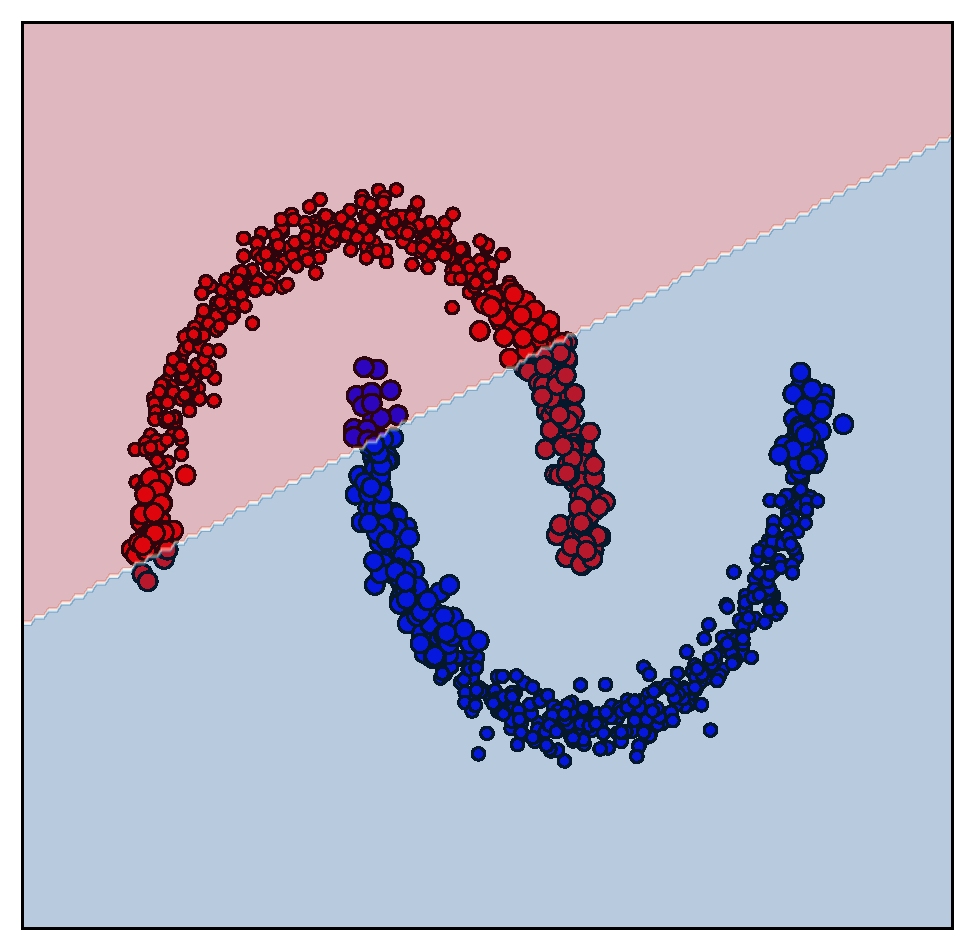
\includegraphics[width=8cm]{../pict/moon_lin.pdf} & 
	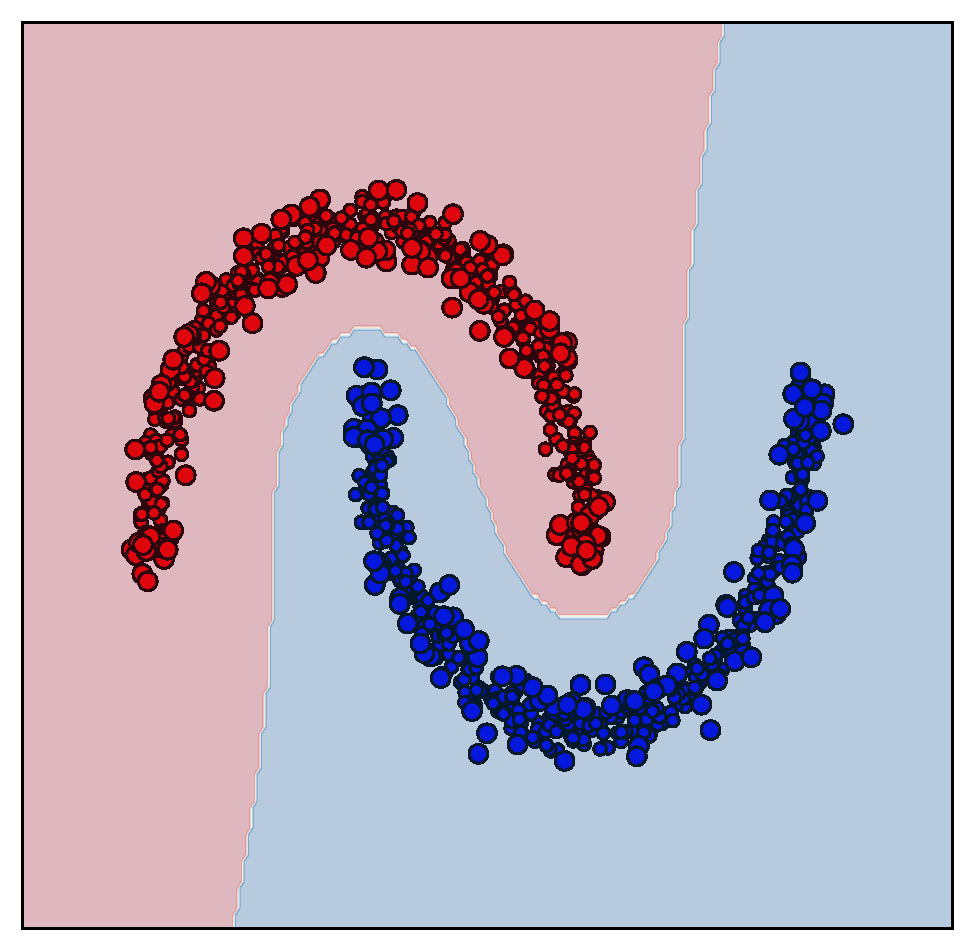
\includegraphics[width=8cm]{../pict/moon_rbf.pdf}
	\\
	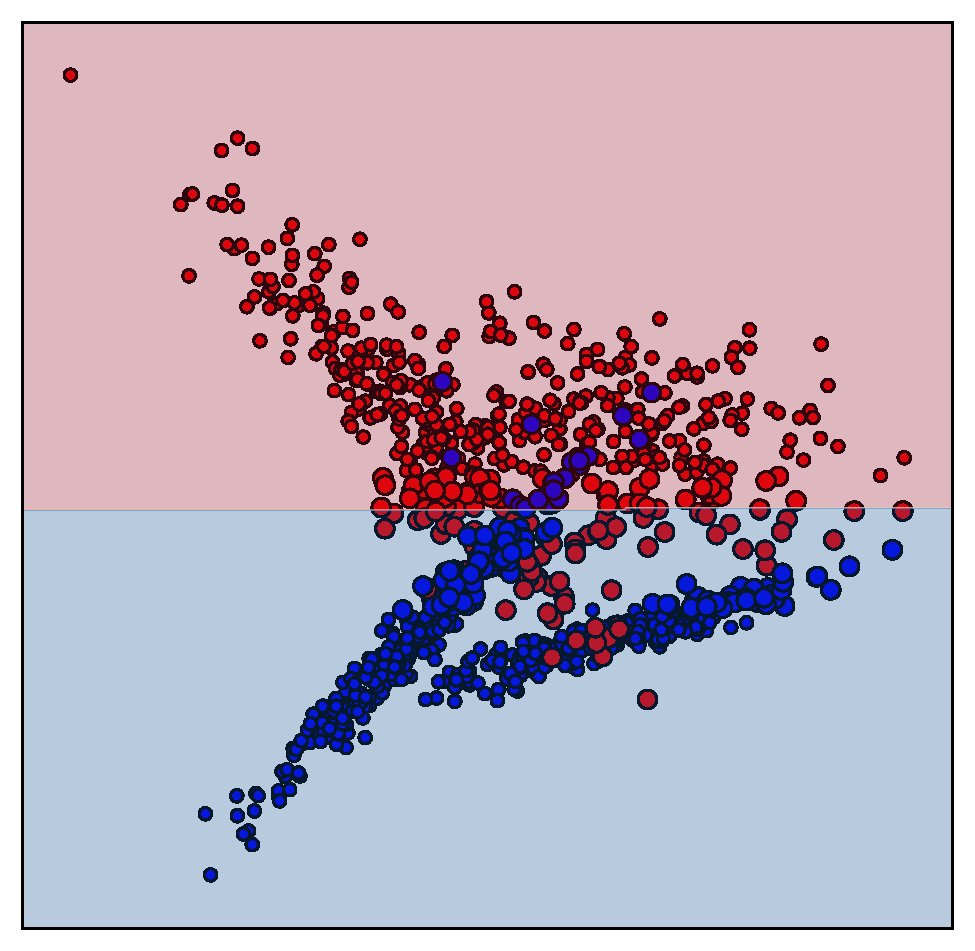
\includegraphics[width=8cm]{../pict/nonsplit_lin.pdf} &
	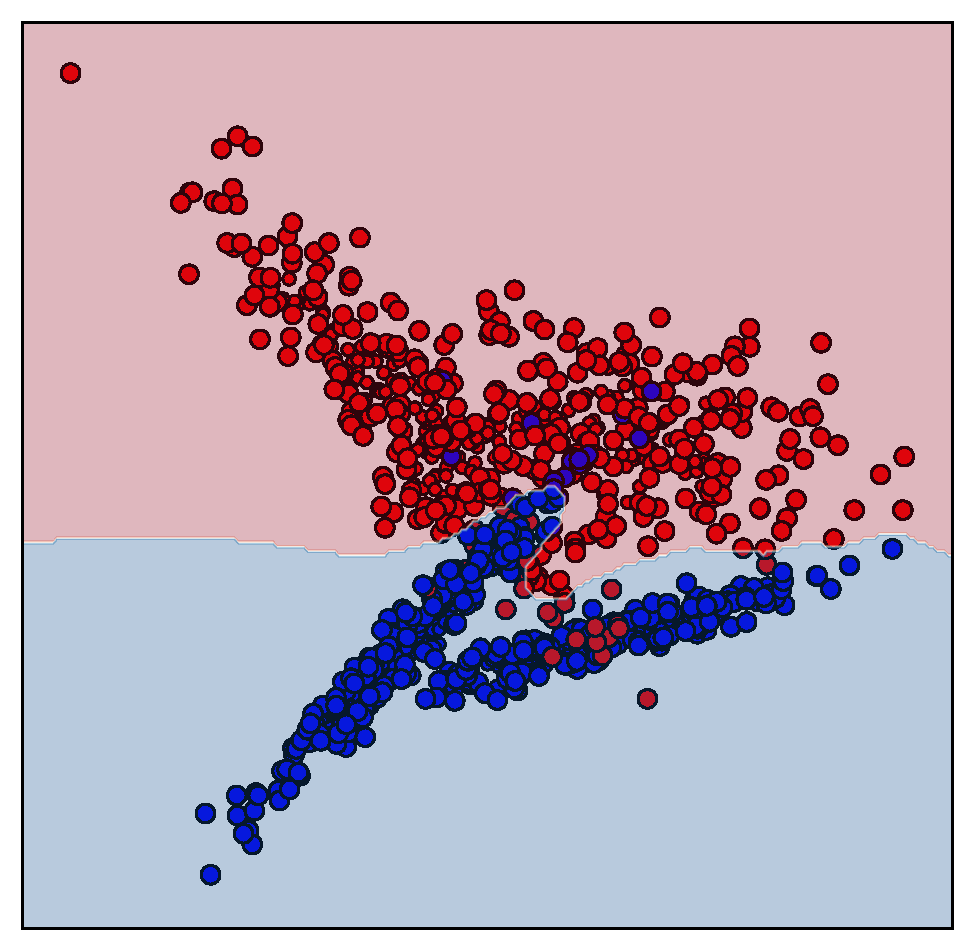
\includegraphics[width=8cm]{../pict/nonsplit_rbf.pdf}
\end{tabular}
\end{figure}

Теперь построим разделяющую поверхность RBF в зависимости от параметра $\gamma$ (Рис. \ref{fig6}).
Параметр $C$ был взят оптимальным, равным $50$.

Видно, что при значениях $\gamma$, больших оптимального, выбросы начинают оказывать большое влияние
на разделяющую поверхность, что уменьшает обобщающую способность алгоритма. При сверхбольших
значениях параметра, граница плотнее прилегает к одному из классов, окольцовывая все его точки, а
все выбросы <<дырявят>> область противоположного класса. Точность классификации на объектах обучающей
выборки в этом случае становится равна $1$, но обобщающая способность такого алгоритма невилика.

\pagebreak
\begin{figure}[h!]
\centering
\caption{Разделяющая поверхность линейного SVM и SVM c ядром}
\label{fig6}
\begin{tabular}{cc}
	$\gamma=0.5$ & $\gamma=5$ \\
	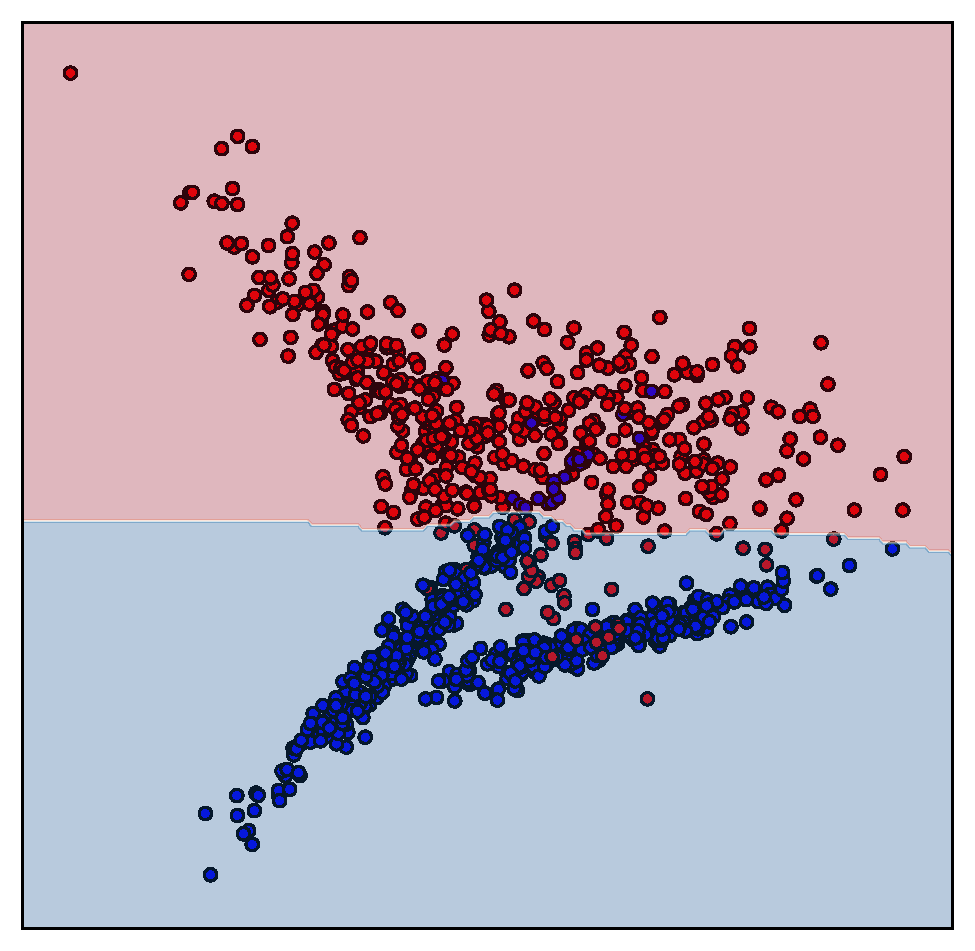
\includegraphics[width=8cm]{../pict/nonsplit_rbf_0.5.pdf} &
	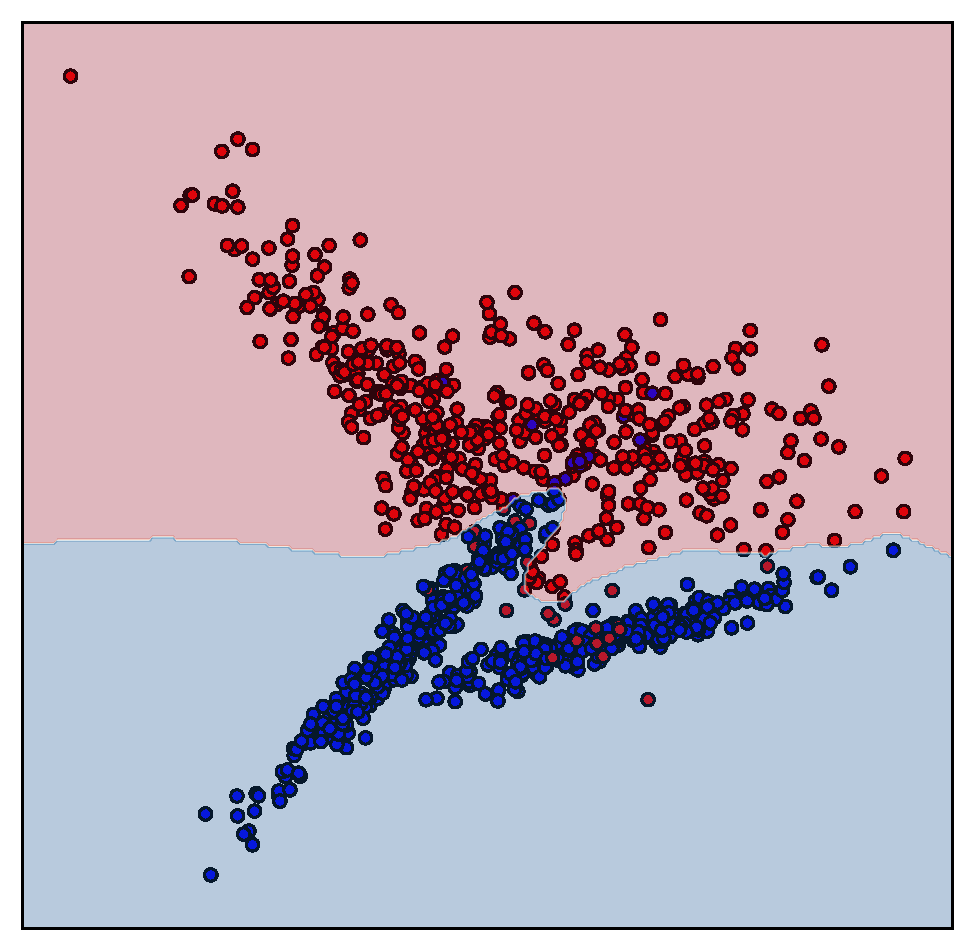
\includegraphics[width=8cm]{../pict/nonsplit_rbf_5.pdf}
	\\
	$\gamma=50$ & $\gamma=500$ \\ 
	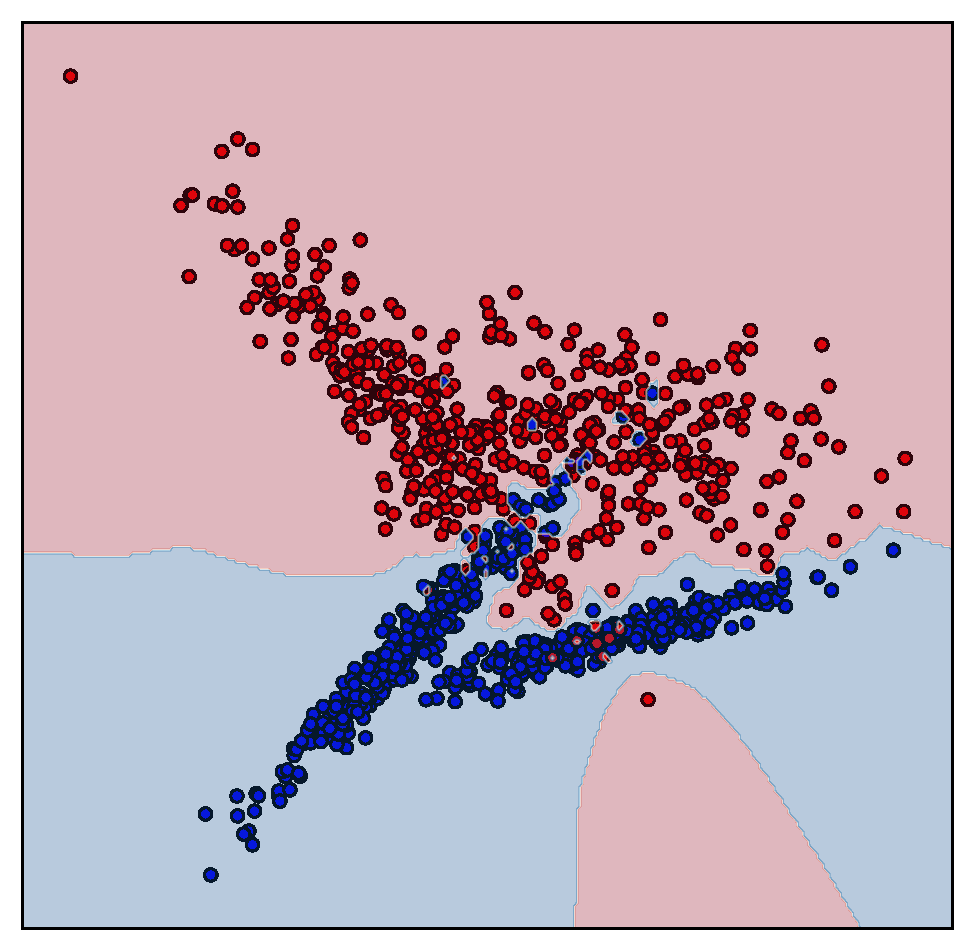
\includegraphics[width=8cm]{../pict/nonsplit_rbf_50.pdf} &
	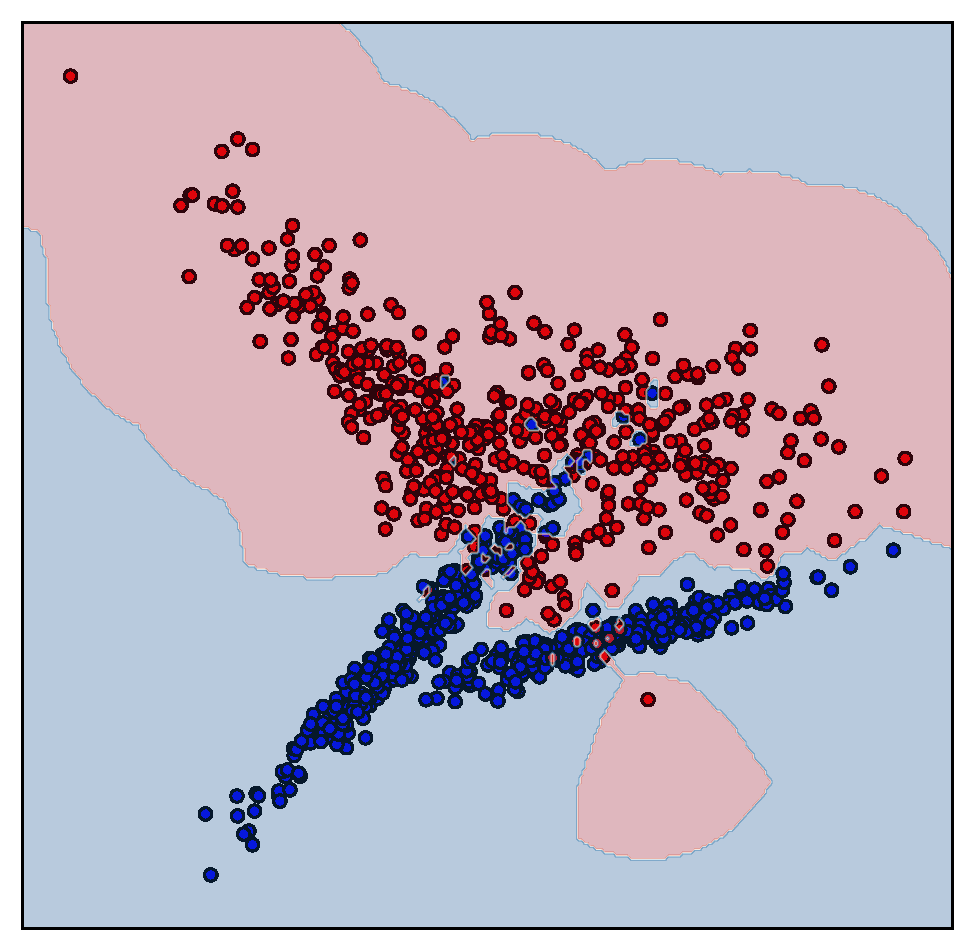
\includegraphics[width=8cm]{../pict/nonsplit_rbf_500.pdf}
\end{tabular}
\end{figure}

\end{document}